\documentclass[a4paper,12pt,oneside]{book}
\documentclass[xcolor=table]{beamer}
%-------------------------------Start of the Preable------------------------------------------------
\usepackage[english]{babel}
\usepackage{blindtext}
\usepackage{longtable}
\usepackage{ltablex}
\usepackage{tabularx}
\usepackage{graphicx}
\usepackage{enumitem}
\setlist{parsep=0pt,listparindent=\parindent}

\usepackage[table,xcdraw]{xcolor}
%packagr for hyperlinks
\usepackage{hyperref}
\hypersetup{
    colorlinks=true,
    linkcolor=blue,
    filecolor=magenta,      
    urlcolor=cyan,
}

\urlstyle{same}
%use of package fancy header
\usepackage{fancyhdr}
\setlength\headheight{26pt}%26
\fancyhf{}
%\rhead{
\includegraphics[width=1cm]{logo}}
\lhead{\rightmark}
\rhead{
\includegraphics[width=1cm]{logo}}
\fancyfoot[RE, RO]{\thepage}
\fancyfoot[CE, CO]{\href{http://www.e-yantra.org}{www.e-yantra.org}}
\renewcommand{\footrulewidth}{0.4pt}

\pagestyle{fancy}

%use of package for section title formatting
\usepackage{titlesec}
\titleformat{\chapter}
  {\Large\bfseries} % format
  {}                % label
  {0pt}             % sep
  {\huge}           % before-code
 
%use of package tcolorbox for colorful textbox
\usepackage[most]{tcolorbox}
\tcbset{colback=cyan!5!white,colframe=cyan!75!black,halign title = flush center}

\newtcolorbox{mybox}[1]{colback=cyan!5!white,
colframe=cyan!75!black,fonttitle=\bfseries,
title=\textbf{\Large{#1}}}

%use of package marginnote for notes in margin
\usepackage{marginnote}

%use of packgage watermark for pages
%\usepackage{draftwatermark}
%\SetWatermarkText{
\includegraphics{logo}}
\usepackage[scale=2,opacity=0.1,angle=0]{background}
\backgroundsetup{
contents={
\includegraphics{logo}}
}

%use of newcommand for keywords color
\usepackage{xcolor}
\newcommand{\keyword}[1]{\textcolor{red}{\textbf{#1}}}

%package for inserting pictures
\usepackage{graphicx}

%package for highlighting
\usepackage{color,soul}

%new command for table
\newcommand{\head}[1]{\textnormal{\textbf{#1}}}


%----------------------End of the Preamble---------------------------------------

%\SetWatermarkText{
\includegraphics{logo.png}}
\begin{document}

%---------------------Title Page------------------------------------------------
\begin{titlepage}
\raggedright
{\Large eYSIP2017\\[1cm]}
{\Huge\scshape \centering{MINIBOT BLOCKLY \\[.1in]}}
\vfill
\begin{flushright}
{\large\textbf{\underline {Intern:}\\}}
{\large Hitesh Tewani \\}
{\large\textbf{\underline {Mentors:}\\}}
{\large Ms. Deepa Avudiappan \\}
{\large Ms. Rutuja Ekatpure \\}
{\large Duration of Internship:   22/05/2017-07/07/2017  \\}
\end{flushright}

{\itshape 2017, e-Yantra Publication}
\end{titlepage}
%-------------------------------------------------------------------------------

\chapter[Project Tag]{MINIBOT BLOCKLY}
\section*{Abstract}
In this report, a web application based Visual Programming Language is proposed for developing a language for easier comprehension of Firebird V code.
This project aims at making expirience of children new to embedded system programming, to grasp the concept of the Alogrithm involved rather than remebering the port configurations.

\section{Introduction and Overview}
The aim of this project is to develop a web application using Laravel Framework and design a Visual Programming Language for Firebird V. Blockly library is used for generating the blocks and parsing them to corresponding C code on the front-end. On the sever side PHP is used for parsing the XML to C code. The final goal of this project is to deliver a web application that contains predefined
blocks for writing the code for Firebird V.

\subsection*{Completion status}
Schematic for MiniBOT along with its modular board schematics are ready. In blockly new blocks for firebird 5 have been successfully added which include Xbee(Tx & Rx), BlueTooth(Tx & Rx) and Servo motor. Development for physical bot is yet not complete.

\\[1cm]
\hfill\includegraphics[width=15cm, height=5cm]{table3}
\\[3cm]
\hfill\includegraphics[width=15cm, height=6cm]{table4}

\section{Hardware parts}
\subsection{List of hardware}

Click \href{https://drive.google.com/open?id=0ByLW6CS6kiaiMDBpdGxDMEZEV0U}{Component List} to view the list of components .
%\hfill\includegraphics[width=15cm, height=18cm]{ct7}
%\\[4cm]
%\hfill\includegraphics[width=15cm, height=19cm]{ct4}
%\\[4cm]
%\hfill\includegraphics[width=15cm, height=19cm]{ct5}

 %\subsection{Description of Components}
 \begin{enumerate}
    \item \textbf{Atmega 2560}\\
    i.Click \href{http://www.atmel.com/Images/Atmel-2549-8-bit-AVR-Microcontroller-ATmega640-1280-1281-2560-2561_datasheet.pdf}{DATASHEET}
    \\[0.5cm]	Atmega2560 is clocked at 14.7456 MHz. It is a 100 pin uC which can be used for multiple purposes.
    
    \\\vspace*{1.3cm}\hspace*{-1cm}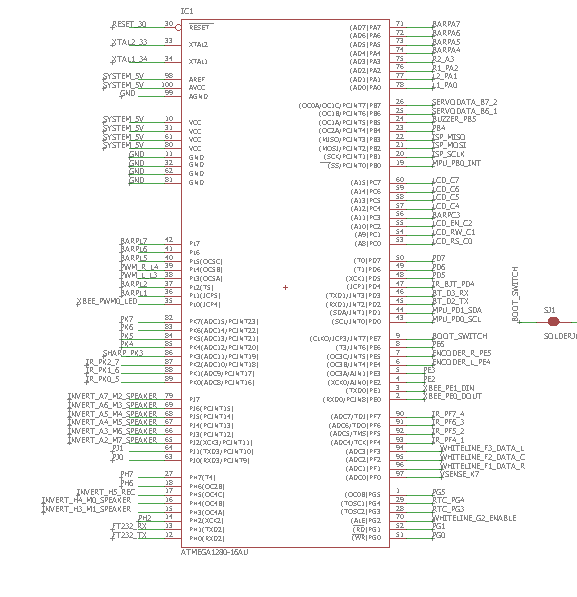
\includegraphics[width=12.5cm, height=18cm]{atmega2560}
    
    
    \newpage\item \textbf{White Line Sensor}\\
    i.Click \href{http://extremeelectronics.co.in/datasheets/IR333C_datasheet.pdf}{DATASHEET}
    \\[0.5cm]Line sensors are used for sensing white line on dark surface or black line on light surface.Line sensor consists of high intensity red LED for illumination and directional photo transistor for line sensing. Phototransistor consists of a photo transistor and convex lens. Because of precise alignment between the lens and photo transistor, it has very narrow viewing angle of 5 degrees. This makes this line sensor highly immune to ambient light. This sensor gives 0.18 volts on bright surface and gives 2.2V or more on the dark surface. Its output is analog in nature. Because of analog output one can write complex algorithm to follow white line using microcontroller.
    We have used three white line sensors,similar to FireBird V. These white line sensors emit red light as red lights frequency which is ideal for detecting contrast between white and black.
    \vspace*{.5cm}
    \\\hfill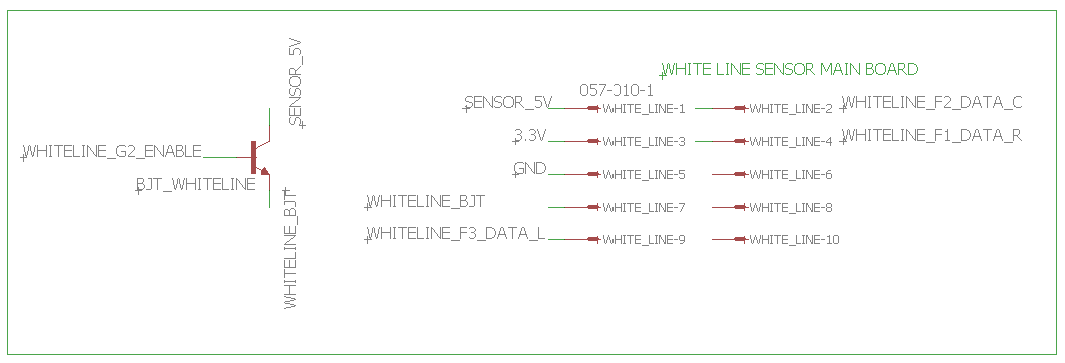
\includegraphics[width=13cm, height=10cm]{Whiteline}
    
    \newpage\item \textbf{Xbee}\\
    i.Click \href{https://www.digi.com/pdf/ds_xbeemultipointmodules.pdf}{DATASHEET}
    \\[0.5cm]MiniBOT uses XBee wireless modules form Digi international (www.digi.com). It supports XBee and XBee Pro wireless modules which gives 100 or 1000+ meters of wireless communication range in line of sight.
    LEDs W1, W2, W3 and W4 are used for status indication of the wireless module. For more details on the wireless module read the wireless module’s datasheet.
    NOTE:
    You can change XBee wireless module’s frequency, and Pan ID so that multiple XBee wireless modules can coexist at the same time. 
    \vspace*{1.5cm}
    \\\hfill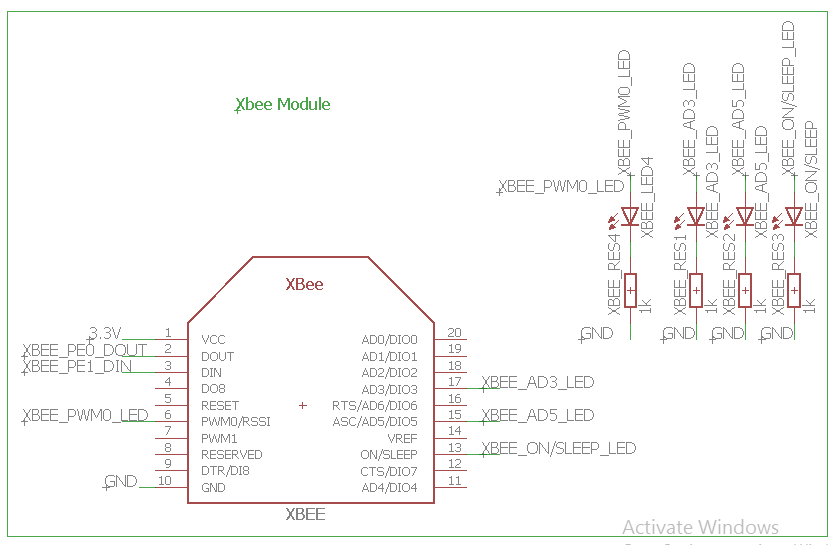
\includegraphics[width=13cm, height=9cm]{Xbee}
    
    \newpage\item \textbf{Crystal Oscillator}\\
    i.Click \href{https://support.epson.biz/td/api/doc_check.php?dl=brief_SG-310SCF_en.pdf}{DATASHEET}
    \\[0.5cm]A crystal oscillator is an electronic oscillator circuit which is used for the mechanical resonance of a vibrating crystal of piezoelectric material. It will create an electrical signal with a given frequency. This frequency is commonly used to provide a stable clock signal and also used to stabilize frequencies for radio transmitters and receivers.
    \vspace*{2.5cm}
    \\\hspace*{3cm}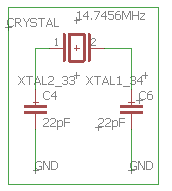
\includegraphics[width=6cm, height=7cm]{Crystal}
    
     \newpage\item  \textbf{TSOP}\\
    i.Click \href{https://www.engineersgarage.com/sites/default/files/TSOP1738.pdf}{DATASHEET}
    \\[0.5cm]TSOP1738 is an IR receiver and RC5 decoder. It is very commonly used in televisions for receiving commands from the remote control. It can be used to control robot using TV remote control. Many robots can be controlled simultaneously if you make your own TV remote equivalent and interface it with the PC. Such type of setup can be used in the preliminary form of robo-soccer. 
    The miniBOT has been provided with a slot to plug the separately provided module for TSOP.\\
    \vspace*{1.5cm}
    \\\hspace*{3.5cm}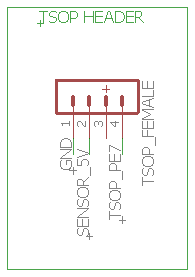
\includegraphics[width=6cm, height=6cm]{TSOP}
    
     \newpage\item \textbf{LCD}\\
    i.Click \href{http://www.vishay.com/docs/37306/lcd016n004b.pdf}{DATASHEET}
    \\[0.5cm]A 16x4 LCD means it can display 16 characters per line and there are 4 such lines. In this LCD each character is displayed in 5x7 pixel matrix. This LCD has two registers, namely, Command and Data. The command register stores the command instructions given to the LCD. A command is an instruction given to LCD to do a predefined task like initializing it, clearing its screen, setting the cursor position, controlling display etc. The data register stores the data to be displayed on the LCD. The data is the ASCII value of the character to be displayed on the LCD. 
    \\\hfill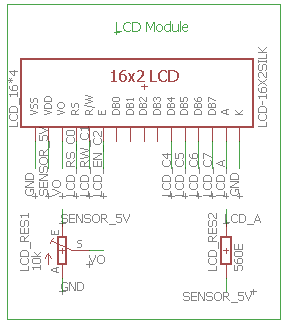
\includegraphics[width=12cm, height=12cm]{LCD}
    
    \item \textbf{IR sensors}\\
    i.Click \href{https://www.vishay.com/docs/83760/tcrt5000.pdf}{DATASHEET}
    \\[0.5cm]An infrared sensor is an electronic device, that emits in order to sense some aspects of the surroundings. An IR sensor can measure the heat of an object as well as detects the motion. The emitter is simply an IR LED (Light Emitting Diode) and the detector is simply an IR photodiode which is sensitive to IR light of the same wavelength as that emitted by the IR LED. When IR light falls on the photodiode, The resistances and these output voltages, change in proportion to the magnitude of the IR light received.
    There are are 7 IR Sensors in all, to give the robot enough degree of perception for avoiding opstacles and managing drives accordingly.
    \\\hfill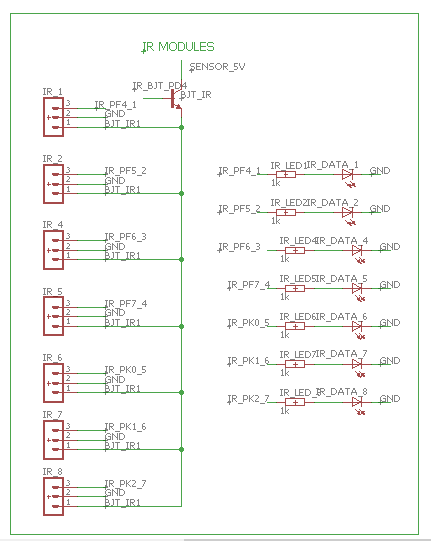
\includegraphics[width=13cm, height=14.5cm]{IR_sensor}
    
    \item \textbf{Servo Motor}\\
    i.Click \href{http://www.es.co.th/schemetic/pdf/et-servo-s3003.pdf}{DATASHEET}
    \\[0.5cm]Servos are controlled by sending an electrical pulse of variable width, or pulse width modulation (PWM), through the control wire. There is a minimum pulse, a maximum pulse, and a repetition rate. A servo motor can usually only turn 90° in either direction for a total of 180° movement. The motor's neutral position is defined as the position where the servo has the same amount of potential rotation in the both the clockwise or counter-clockwise direction. The PWM sent to the motor determines position of the shaft, and based on the duration of the pulse sent via the control wire; the rotor will turn to the desired position. The servo motor expects to see a pulse every 20 milliseconds (ms) and the length of the pulse will determine how far the motor turns. For example, a 1.5ms pulse will make the motor turn to the 90° position. Shorter than 1.5ms moves it in the counter clockwise direction toward the 0° position, and any longer than 1.5ms will turn the servo in a clockwise direction toward the 180° position. When these servos are commanded to move, they will move to the position and hold that position. If an external force pushes against the servo while the servo is holding a position, the servo will resist from moving out of that position. The maximum amount of force the servo can exert is called the torque rating of the servo. Servos will not hold their position forever though; the position pulse must be repeated to instruct the servo to stay in position. 
    \\\hfill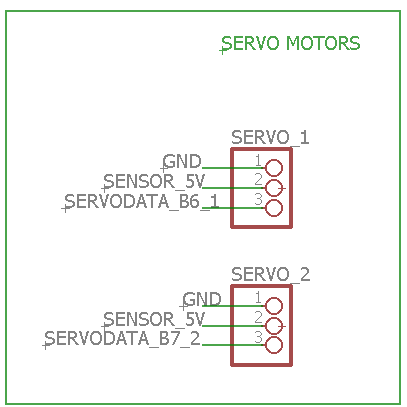
\includegraphics[width=12cm, height=10cm]{servo}
    
    
    
    \item \textbf{Bluetooth}\\
    i.Click \href{http://www.electronicaestudio.com/docs/istd016A.pdf}{DATASHEET}
    \\[0.5cm]HC‐05 module is an easy to use Bluetooth SPP (Serial Port Protocol) module, designed for transparent wireless serial connection setup. The HC-05 Bluetooth Module can be used in a Master or Slave configuration, making it a great solution for wireless communication. This serial port bluetooth module is fully qualified Bluetooth V2.0+EDR (Enhanced Data Rate) 3Mbps Modulation with complete 2.4GHz radio transceiver and baseband. It uses CSR Bluecore 04‐External single chip Bluetooth system with CMOS technology and with AFH (Adaptive Frequency Hopping Feature).
    MiniBOT has been provided with a separate 4 pin outs to use bluetooth by simply pluging it. We can also add more than one blutooth module on the GPIO ports provided separately.
    \\\hfill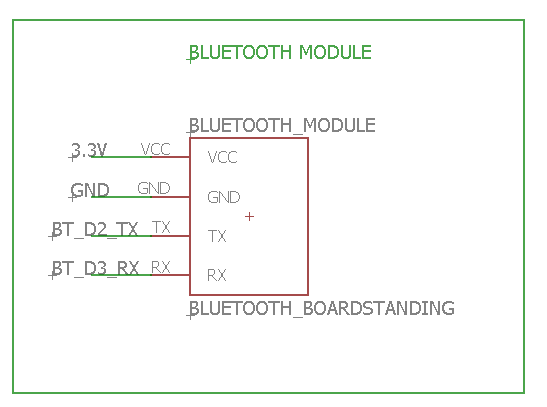
\includegraphics[width=12cm, height=10cm]{bluetooth}
    
    \newpage\item \textbf{ISP Header}\\
    i.Click \href{http://www.cs.ou.edu/~fagg/classes/general/atmel/avrisp_ug.pdf}{DATASHEET}
    \\In-system programming (ISP), also called in-circuit serial programming (ICSP), is the ability of some programmable logic devices, microcontrollers, and other embedded devices to be programmed while installed in a complete system, rather than requiring the chip to be programmed prior to installing it into the system.
    MiniBOT blockly has been provided with a Header which can be used to program the Atmega2560 Microcontroller using ISP programming.
    \vspace*{1.5cm}
    \\\hspace*{.5cm}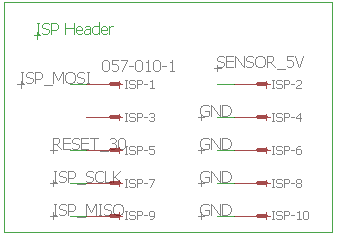
\includegraphics[width=12cm, height=9.5cm]{isp}
    
    \newpage\item \textbf{MPU6050}\\
    i.Click \href{https://www.invensense.com/wp-content/uploads/2015/02/MPU-6000-Datasheet1.pdf}{DATASHEET}
    \\[0.5cm]The MPU6050 has an embedded 3-axis MEMS gyroscope, a 3-axis MEMS accelerometer. It is very useful for some motion detecting. We have provided pinouts for placing the MPU6050 on the MiniBOT. This module is compatible with 3.3v as well as 5 volt supply, but in our BOT we have provided it with the 5v supply.
    \vspace*{1.5cm}
    \\\hspace*{.5cm}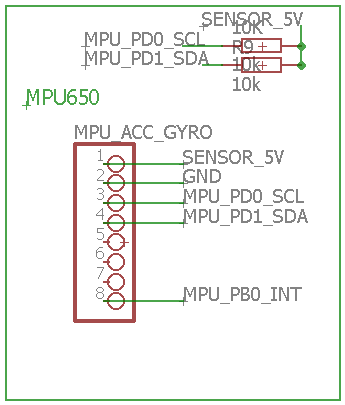
\includegraphics[width=12cm, height=12cm]{Mpu6050}
    
    \newpage\item \textbf{Power Management}\\
    i.Click \href{http://www.ti.com/lit/sg/slvt145q/slvt145q.pdf}{Power Management Guide}
    \\[0.5cm]MiniBOT is powered by 9.6V, 2.1Ah rechargeable Nickel Metal Hydride battery pack. When it is fully charged, battery pack gives 11.5V. When it is fully discharged, voltage drops to about 8.5V. Battery pack should not be discharged below 8V (1V per cell) for extended battery life. Nickel Metal Hydride batteries must be recharged using smart charging circuit which follows the appropriate charging profile for the batteries. To avoid any damage to the batteries, only use the charger provided with the robot. 
    Power Management circuit has been provided with various regulators like 7805 and LD1117 to bring down the voltage to a level which is desired by each circuit.
    
    \\\hspace*{-1.5cm}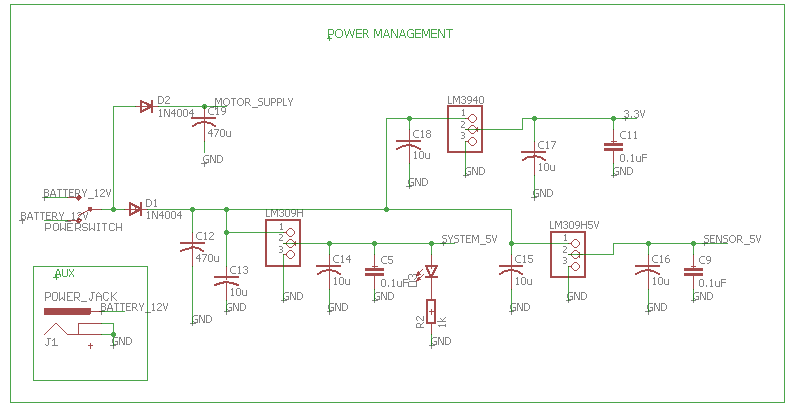
\includegraphics[width=15cm, height=13cm]{powermanage}
    
    \newpage\item \textbf{Battery Voltage Sensing}
    \\[0.5cm]These are connected to the ADC pins of the microcontroller.
    Filtered battery voltage is used for battery voltage sensing. Analog to Digital Converter (ADC) can measure maximum voltage of 5V. Hence battery voltage is scaled down from 8-15V to less
    than 5V using resistor divider network formed by R12 and R13. It scales down the voltage by approximately 1/3 of the actual value. ATMEGA2560 ADC can be used in 8 bit or 10 bit resolution.
    To calculate voltage from the ADC’s acquired digital value in 8 bit resolution we use following formula:\\
    V Battery = 0.7V + (ADC value * (5V/255) * ((10K + 3.3K) / 3.3K))\\
    V Battery = 0.7V + (ADC value * 0.0790)\\
    In the above formula:\\
    a) 0.7V represents voltage drop across the diodes. For more details refer to the figure.\\
    b) 5V/255 represents the ADC step resolution\\
    c) (10K + 3.3K) / 3.3K is a voltage divider formula
    \vspace*{1cm}
    \\\hfill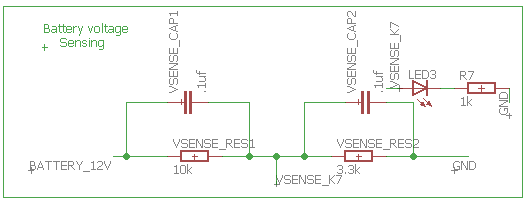
\includegraphics[width=12.5cm, height=8cm]{bvs}
    
     \newpage\item \textbf{Boot Switch}\\
     \\It makes use of a push button switch to give user inputs to the microcontroller.
     \vspace*{1.5cm}
    \\\hspace*{1cm}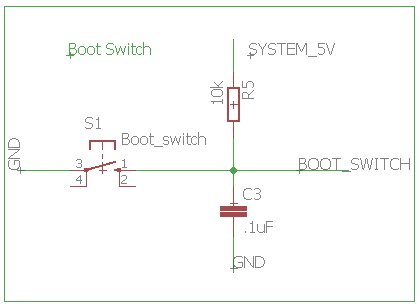
\includegraphics[width=11cm, height=9cm]{boots}
    
     \newpage\item \textbf{L293D connector}\\
    i.Click \href{http://www.ti.com/lit/ds/symlink/l293.pdf}{DATASHEET}
    \\[0.5cm]Motion control involves direction control and velocity control. Motors are controlled by L293D dual motor driver which can provide up to 600mA of current to each motor. To change the
    direction of the motor, appropriate logic levels (High/Low) are applied to L293D’s direction control pins. Velocity control is done using Pulse Width Modulation (PWM). 
    L293D is connected below the MiniBOT along with encoders.
    \vspace*{1cm}
    \\\hspace*{0.6cm}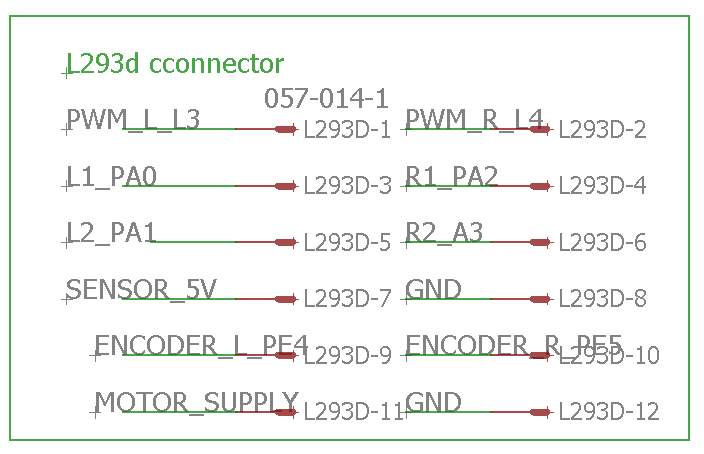
\includegraphics[width=12cm, height=11cm]{l293d1}
    
    \newpage\item \textbf{Speaker}\\
    i.Click \href{https://img.ozdisan.com/ETicaret_Dosya/358195_3955320.pdf}{DATASHEET}
    \\[0.5cm]It can record and play upto 8 voice messages and can store messages upto 11 minutes at 8KHz sampling rate.
    It has a powerful 16-Bits Digital Audio Processor with nonvolatile Flash Memory Technology.
    The miniBot is designed to play 4 inbuilt predefined sounds like ambulance,rhymes etc and three user defined sounds which would be recorded by the user. One pin has been reserved to play the sound "Hi, I am Blockly", every time the bot restarts.
    \vspace*{1cm}
    \\\hspace*{.4cm}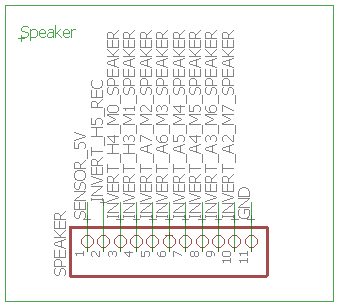
\includegraphics[width=12cm, height=11cm]{Speaker}
    
    \newpage\item \textbf{Reset}\\
    \\\hfill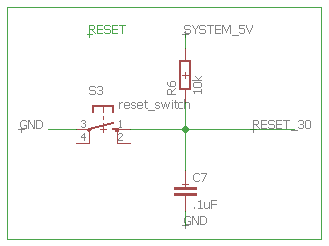
\includegraphics[width=12cm, height=11cm]{RESET}
    
    \newpage\item \textbf{Sharp Sensors}\\
    i.Click \href{https://www.sparkfun.com/datasheets/Sensors/Infrared/gp2y0a02yk_e.pdf}{DATASHEET}
    \\[0.5cm]Sharp sensor add more resolution to the measurement of obstacles. 
    Only one sharp sensor slot has been provided where sensor can be plugged and used. The sharp sensor is in front of the bot and has a range of 10 to 80 cm's. 
    \vspace*{1.5cm}
    \\\hfill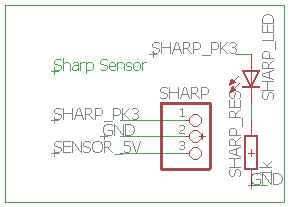
\includegraphics[width=12cm, height=10cm]{sharp}
    
    
    \newpage\item \textbf{GPIO Ports}\\
    i.Click \href{https://www.sparkfun.com/datasheets/Sensors/Infrared/gp2y0a02yk_e.pdf}{DATASHEET}
    \\[0.5cm]Minibot has 30 GPIO ports which consist of various ADC pins,UART pins and other general purpose pins along with pins for ground and power supply i.e 3.3v & 5v.
    \\30 empty GPIO ports have been provided for future use.
    \\\hfill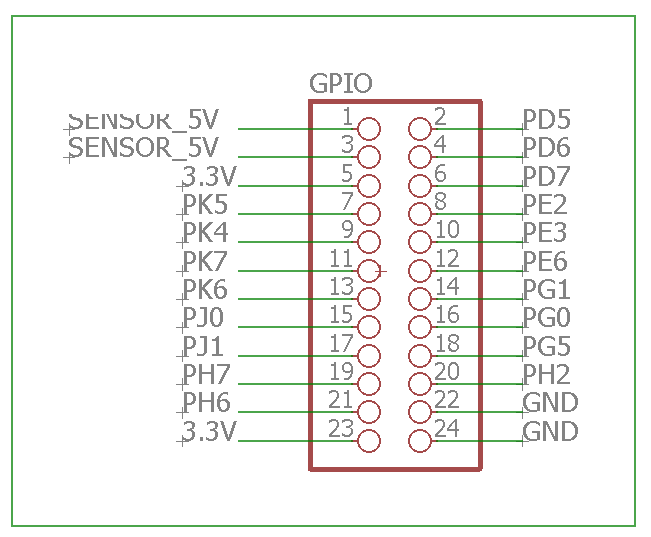
\includegraphics[width=12cm, height=15cm]{GPIO}
    
   \newpage \item \textbf{Encoders & L293d}\\
    i.Click \href{http://www.datasheetspdf.com/datasheet/MOC7811.html}{DATASHEET}
    \\[0.5cm]Position encoders give position / velocity feedback to the robot. It is used in closed loop circuits to control robot’s position and velocity. Position encoder consists of slotted disc which rotates between optical encoder (optical transmitter and receiver). When slotted disc moves in between the optical encoder we get square wave signal whose pulse count indicates position and time period / frequency indicates velocity.Optical encoder MOC7811 is used for position encoder on the robot. It consists of IR LED and the photo transistor mounted in front of each other separated by a slot in black opaque casing with small slot shaped window facing each other.
    When IR light falls on the photo transistor it gets in to saturation and gives logic 0 as the output. In absence of the IR light it gives logic 1 as output. A slotted encoder disc is mounted on the wheel which is placed in between the slot. When encoder disc rotates it cuts IR illumination alternately because of which photo transistor gives square pulse train as output.
    \\Two positional encoders have been used which help in tracking the position, angle and speed of the robot.
    \\\hfill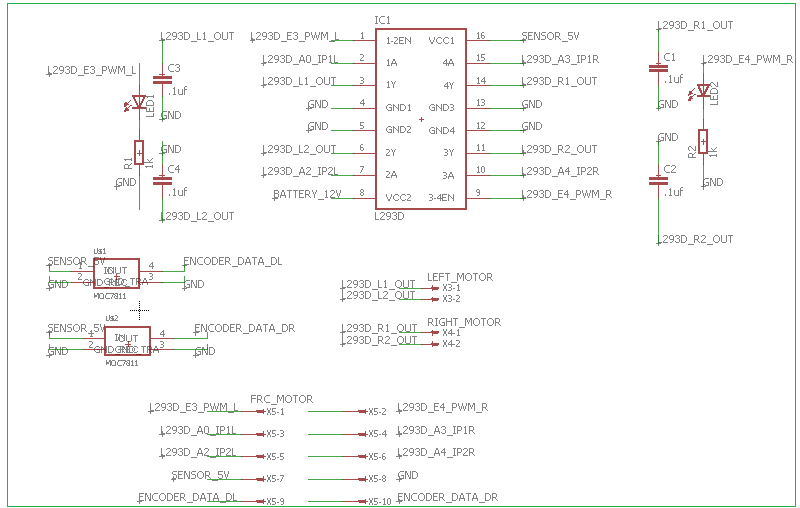
\includegraphics[width=13cm, height=10cm]{enc}
    
    
    \newpage\item \textbf{Battery Supply}\\
    i.Click \href{https://system.netsuite.com/core/media/media.nl?id=1760870&c=1327152&h=aaae2543a511565767bc&_xt=.pdf}{DATASHEET}
    \\\hspace*{3cm}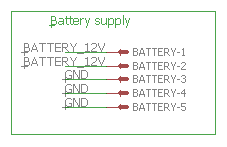
\includegraphics[width=6cm, height=6cm]{btsu}
    
     
    \item \textbf{USB Type C Port Connection}\\
    \\\hfill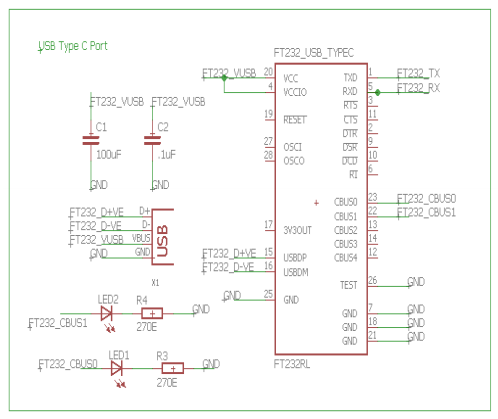
\includegraphics[width=13cm, height=11cm]{usbc}
    
 \end{enumerate}
 %1.Atmega 2560\\
  %\href{http://www.atmel.com/Images/Atmel-2549-8-bit-AVR-Microcontroller-ATmega640-1280-1281-2560-2561_datasheet.pdf}{DATASHEET}
 
 % \item Detail of each hardware: %\href[page=5]{./datasheet/MPU-9150.pdf}{Datasheet, page 5}, %\href{http://www.amazon.in}{Vendor link}, 
  %\item Connection diagram


%\subsection{List of hardware}


\newpage\section{Software used}
The Blockly library has been used which is based on MVC Framework(Model View Controller).
The Model-View-Controller (MVC) is an architectural pattern that separates an application into three main logical components: the model, the view, and the controller.
\begin{itemize}
\item{Model}\\
The Model component corresponds to all the data-related logic that the user works with. This can represent either the data that is being transferred between the View and Controller components or any other business logic-related data. For example, a Customer object will retrieve the customer information from the database, manipulate it and update it data back to the database or use it to render data.\\
In our Blockly,MySQL cloud service and phpMyAdmin come under Model Framework.
\item{View}\\
The View component is used for all the UI logic of the application. For example, the Customer view will include all the UI components such as text boxes, dropdowns, etc. that the final user interacts with.\\
HTML,PHP,CSS,Javascript and Ajax can be classified under the View Framework.
\item{Controller}\\
Controllers act as an interface between Model and View components to process all the business logic and incoming requests, manipulate data using the Model component and interact with the Views to render the final output. For example, the Customer controller will handle all the interactions and inputs from the Customer View and update the database using the Customer Model. The same controller will be used to view the Customer data.\\
JSON and jQuery come under Controller framework.
\end{itemize}

\begin{itemize}
  %\item List of software used 
  %\item Detail of software: version, %\href{http://www.amazon.com}{download link}, 
  %\item Installation steps
  \subsection{What is Blockly}
  Blockly is a client-side JavaScript library for creating visual block programming languages and editors. It is a project of Google and is open-source under the Apache 2.0 License. It typically runs in a web browser, and visually resembles Scratch. Blockly has also been implemented for Android and iOS; though not all web browser based features are available for Android/iOS.
  Blockly uses visual blocks that link together to make writing code easier, and can generate JavaScript, Python, PHP or Dart code. It can also be customised to generate code in any textual computer language.\\[0.5cm]
  \\\hfill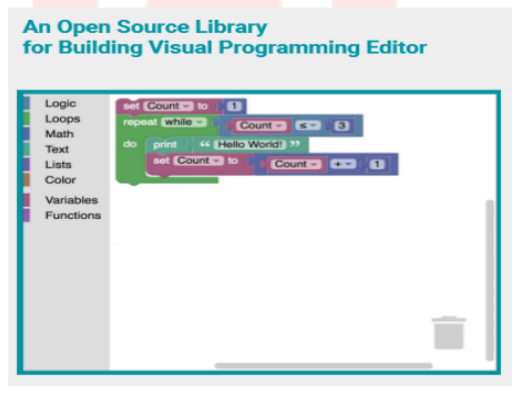
\includegraphics[width=12cm, height=9cm]{imag1}\\[0.5cm]
  \begin{itemize}
    \item\textbf{User interface}
    The default user interface of the Blockly editor consists of a toolbox, which holds available blocks, and a workspace, where the user can drag (from the toolbox) and rearrange blocks. The workspace also includes, by default, zoom icons and a trashcan for deleting blocks. Note that the editor can be customised by visual language developers to customise the editing features available, as well as limiting which blocks are available.
  \end{itemize}
  \subsection{Installing Composer, Laravel, Blockly, Xampp}
  \begin{itemize}
      \item \textbf{Composer}\\
      Run this in your terminal to get the latest Composer version:\\
	\textbf{curl -sS https://getcomposer.org/installer | php\\
      Or if you don't have curl:}\\
	 \textbf{php -r "readfile('https://getcomposer.org/installer');" | php}\\
      This installer script will simply check some php.ini settings, warn you if they are set incorrectly,\\
      and then download the latest composer.phar in the current directory.\\      
      After downloading the composer, Windows Users must set the environment path of the composer.
      For Ubuntu executed \textbf{php composer.phar install} command to install.
      \newpage
      \item \textbf{Xampp}\\
      \begin{itemize}
      \item 
      For installing the xampp application in Windows OS it is first needed to download the executable file.
      To download the installer file, go to\\ \textbf{https://www.apachefriends.org/download.html}\\\href{https://www.apachefriends.org/download.html}{Click Here}
      and download the appropriate file based on the operating system running. 
      \item
      The Xampp application is a Apache, MySql and PHP server used for running webapplications or webpages on the 
      localhost. The Xampp application provides with many other features like executing the applications that are already
      installed on the machine. 
      \item
      For launching any web application or web page on the server, it is first required to copy the folder containing the Webpages to the Xampp/htdocs folder. Then go to Xampp Control Panel and start the Apache and MySQL services. Now go to web browser and type\\\textbf{localhost/Folder/index.html} or for Laravel Framework type\\ \textbf{localhost/folder/public/}
      \end{itemize}
      \newpage
      \item \textbf{Laravel}
      \begin{itemize}
	\item
	Laravel Framework is a PHP5 Framework used for website designs which give a structured directory arrangement. 
	Laravel attempts to take the pain out of development by easing common tasks used in the majority of web projects,
	such as authentication, routing, sessions, queueing, and caching.
	\item 
	Installing Laravel requires composer which is previously installed. Just go to terminal and type the folllowing command,\\
	\textbf{composer global require "laravel/installer=~1.1}\\
	This command installs the Laravel on the machine.
	\item
	If the framework is to be included in a project the type the command,\\
	\textbf{composer create-project laravel/laravel --prefer-dist}\\ wherein the framework is directly installed while creating a project.
	\item 
	After Installing Laravel there may be permission issues for accessing the files. Inorder to solve these problem, change the file permissions for
	storage directory by typing \\\textbf{chmod -R 777 /storage} by going in project directory.\\
      \end{itemize}
      \newpage
      \item \textbf{Blockly}
      \begin{itemize}
	\item
	Blockly is a library for using Visual Programming Language editors. Blockly is javascript library, using which one can
	create and define various block for a Visual Programming Language.
	\item
	To download Blockly goto,\\ \textbf{https://developers.google.com/blockly/installation/o\\verview}\\
	\href{https://developers.google.com/blockly/installation/overview}{Click Here}
	and download from one of the three options.
	\item 
	Blockly provides generation of syntax for Javascript, Python and Dart. However any language code can be generated by 
	modifying the generators file appropriately.
	\item 
	The Library is used for mostly frontend parsing of the blocks to required code. These blocks make up a programming language that was designed around a set of principles to engage novice programmers.\\
      \end{itemize}
  \end{itemize}
  \newpage

\end{itemize}

\subsection{Defining Blocks, as in Visual Programming Language}
\\\hfill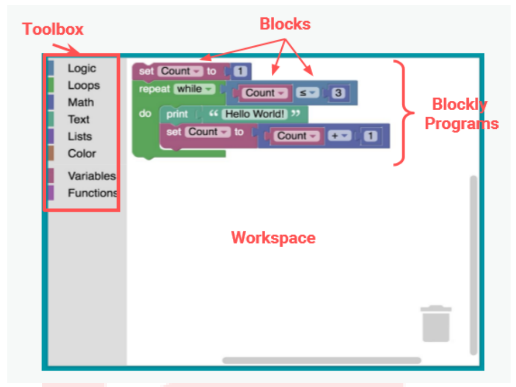
\includegraphics[width=12cm, height=9cm]{imag2}\\[0.5cm]
  \begin{itemize}
   \item \textbf{Creating Blocks}\\
    \begin{itemize}
      \item 
      To generate the blocks, google-blockly provides a block-factory site where, one can easily create the blocks with desired input and names and view them.
      \item
      The block-factory provides the developer with a javascript code for the block created. This code can then added to the blocks folder in a file.
      \item
      The Visual Programming Language consisted of the custom blocks for Firebird V like forward, buzzer, left\_degrees etc. All these 
      blocks were generated and add to the blockly library using the factory.
      \item 
      Once the blocks are created they need to be stored in blocks folder. To view a block on the index page, the block tag
      is to be added to index.html file with tag type as block name.
    \end{itemize}
    
    \begin{center}
      \hspace*{-2cm}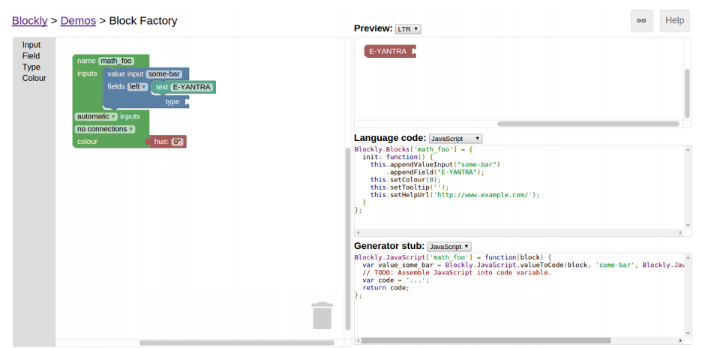
\includegraphics[scale = 0.85]{imag3}\\
      \textbf{ Block Factory} %3.1
    \end{center}
    \newpage
   \item \textbf{Creating Generators}\\
    \begin{itemize}
      \item
      As Blockly provides Javascript code for wach block, in the same it also provides Javascript code for parsing these blocks to requires language.
      \item
      However the Javascript genrator files provided by blockly are only for Javascript, Python and Dart.
      \item
      To make the generator files, it is necessery to know the functions related to each in the block.
      Blockly defines three such function for taking the values from the Inputs.
	\begin{itemize}
	 \item {getFieldValue(var name)}..
	 \item {valueToCode(var block, var name, var precedence)}..
	 \item {statementToCode(var block, var name)}..
	\end{itemize}
      \item
      Using these functions, values of other blocks attached to the current block can be obtained.\\
    \end{itemize}
  \end{itemize}
  \newpage
\subsection{XML Parsing to C Code}
  \begin{itemize}
	\item
	For creating XML to C syntax on the server side a PHP controller is defined in which all the functions are written.
	After adding new blocks, corresponding C syntax for block on the server side is written in ParseController.php. 
	\item
	Each block contains a xml script and connecting blocks creates the corresponding script. This Xml script is used for parsing to C code on the server side.
	\item
	For XML to C parsing there are some functions similar to that in Javascript used for getting the values from connected blocks.
	 \begin{itemize}
	   \item\textbf{function xmlToCode(\$xmlDoc){...}}\\
	   Above function basically finds the childs of node and according to the no of child node, for each child node it calls the blockToCode() function,which finds the type of block (whether it is control\_if block or if\_else block etc) and calls the functions finds the type of input that it takes (like whether it takes getFieldInput() where user give the input or statementToCode() where user gives the proper statement as a input or valueToCode() where user connect some another block to given block as input) , according to that it return the equivalent parsed c code to parse function for the further process.\\
	   \item\textbf{function getFieldValue(\$block,\$name){...}}\\
	   Above function takes two input namely \$block,\$name .\$name basically gives the attribute of field node with the help of that one can find the value of input field .\\
	   \item
	   \textbf{function valueToCode(\$block,\$name){...}}\\
	   Above function takes two input namely \$block ,\$name. valueToCode() function basically takes a block as a input,so after finding the proper child of given parent node blockToCode() function called for further process.\\
	   \item\textbf{function statementToCode(\$block,\$name){...}}\\
	   Above function basically takes two arguments i.e \$block,\$input and finds the statement node and correspondingly find the value of that node.e.g control\_if blog.\\
	 \end{itemize}
  \end{itemize}
\subsection{Execute, Save and Open \\ Button for both XML and C code}
   Whenever the user creates a project using Fireblock he/she should be able to save and restore the project. For this purpose button like
   \begin{itemize}
     \item \textbf{Save XML}\\
      This button allows the user to save the XML file to users Desktop and provide them for later use.
      The xml file is stored using a javascript code save.js
     \item \textbf{Open XML}\\
     To restore the previous project the user can upload the xml file to the server and the server then can restore the blocks that the user had been working on.
     To do so we make use of openButton javascript code which opens the dialogue for s
     \item \textbf{Save C}\\
     Once the user has finished implementing the algorithm he/she can save the C code visible in FirebirdV Tab into file on the local machine
     \item \textbf{Execute}\\
     Once the algorithm is implemented using the blocks the user can then verify and click the Execute button and then if the alogrithm is free of errors
     then a hex file will be made available for download. Clicking this button executes a parse.js function in which send the xml text to the server for parsing.
   \end{itemize}
\newpage
\subsection{Making a compiler to convert C file to hex and allowing it be downloaded} 
    The main task of the web application is to provide a hex file to download. To do so, after completing the impletmentation of the the algorithm,
    user clicks on the execute button; this sends the control to parse.js after compiling. 
    
\subsection{Using Blockly}
    In this Project we have used Laravel Framework for efficient and elegant handling of server.
    On opening the Webpage of this site, it redirects to Fireblocks.blade.php. Using Blade Templating the header contents are defined in FireBlocks.blade.php
    and the main body is contained in blocks.blade.php. The blocks.blade.php file contains the html code for blocks that are visible.
    The blocks are divided into categories which are named according to their types. \\
    The Web application is divided into 3 phases-
    \begin{itemize}
     \item Blocks
     \item Front End C Code.
     \item Back End C Code.
    \end{itemize}
    The workflow of the application goes through all this 3 phases for final hex file generation.\\
   \subsection{Blocks}
    In this phase the the user designs the algorithm using the predefined blocks that are provided on the side tab.
    This blocks when dragged onto the workspace, an xml code is generated in tandem of corresponding block which gives information regarding the same.\\
    XML provides information about each block and the structure of the XML  gives the information about the connections of the blocks.
    \begin{center}
    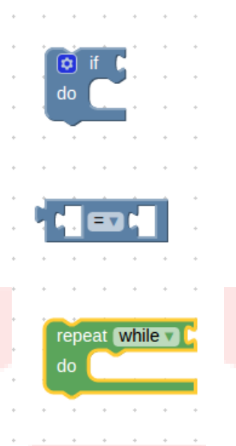
\includegraphics[scale =0.6]{imag5}\\[.3in]
    \textbf{Blocks on Workspace}\\[1.3in]
    \end{center}

    \begin{center}
    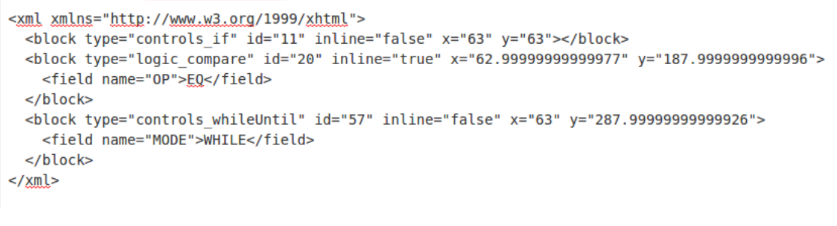
\includegraphics[scale =0.5]{imag6}\\[.3in]
    \textbf{Corresponding XML Syntax}
    \end{center}
    \newpage
    \subsection{Front-End C Code}
    After the user has finished with the algorithms using blocks he/she can verify the code formed by the blocks.
    FirebirdV tab when clicked displays the C code genrated by the blocks. This code is structured according to the XML structure.
    Front End  C code parsing is done by using Blockly library. \\
    
    \begin{center}
    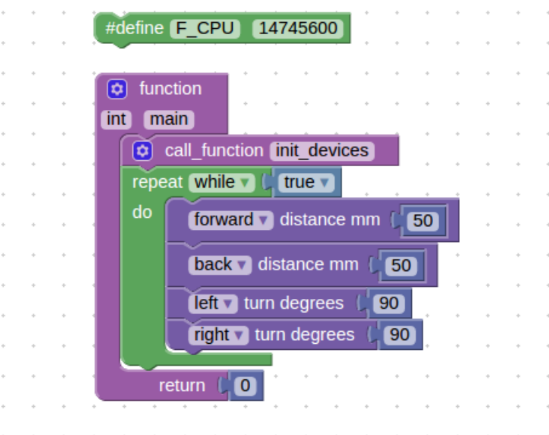
\includegraphics[scale =0.6]{imag7}\\[.1in]
    \textbf{Blocks on Workspace}\\[1in]
    \end{center}

    \begin{center}
    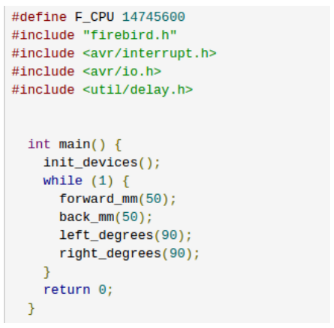
\includegraphics[scale =0.5]{imag8}\\[.1in]
    \textbf{Corresponding C Syntax}
    \end{center}
    
    \newpage\begin{center}
    \section{Blocks added to firebird 5 Blockly}
    \end{center}
    
    \begin{center}
    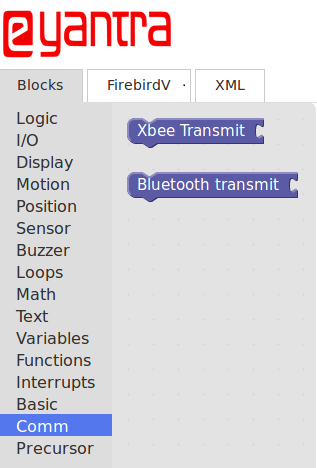
\includegraphics[scale =0.6]{xbtransm}\\[.3in]
    \textbf{Bluetooth and Xbee transmit}\\[1.3in]
    \end{center}
    
    \begin{center}
    \vspace*{-2cm}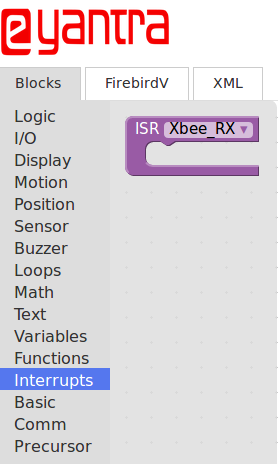
\includegraphics[scale =0.6]{xbrec}\\[.3in]
    \textbf{Bluetooth and Xbee receive}\\[1.3in]
    \end{center}
    
    \begin{center}
    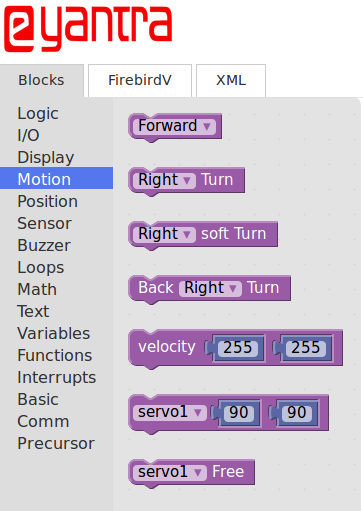
\includegraphics[scale =0.6]{servob}\\[.3in]
    \textbf{Servo and Servo free}\\[1.3in]
    \end{center}
    
    \begin{center}
    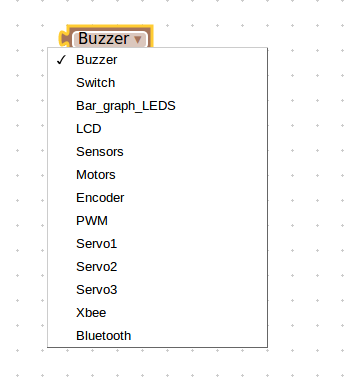
\includegraphics[scale =0.6]{initb}\\[.3in]
    \textbf{Initialization Block Updated}\\[1.3in]
    \end{center}
    
    \begin{center}
    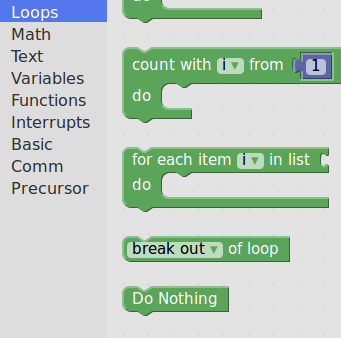
\includegraphics[scale =0.6]{Dono}\\[.3in]
    \textbf{Do Nothing}\\[1.3in]
    \end{center}
    
\newpage\begin{center}
    \section{Examples of Blocks Added}
    \end{center}
    
\begin{center}
    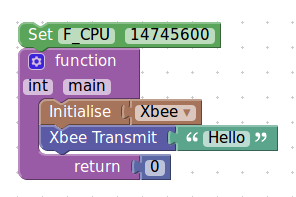
\includegraphics[scale =0.6]{xbeetxsam}\\[.3in]
    \textbf{Xbee Transmit}\\[1.3in]
    \end{center}
    
\begin{center}
    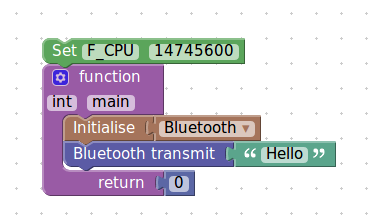
\includegraphics[scale =0.6]{blutxsam1}\\[.3in]
    \textbf{Bluetooth Transmit}\\[1.3in]
    \end{center}
    
\begin{center}
    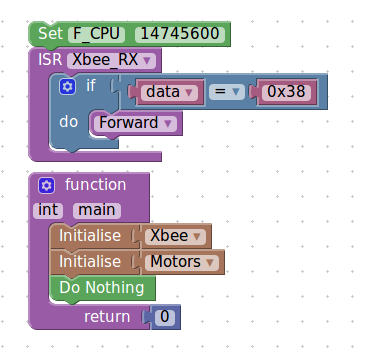
\includegraphics[scale =0.6]{xbeerecimp}\\[.3in]
    \textbf{Xbee Receive}\\[1.3in]
    \end{center}
    
\begin{center}
    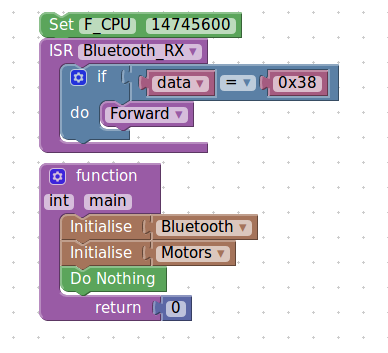
\includegraphics[scale =0.6]{blerecimp}\\[.3in]
    \textbf{Blutooth Receive}\\[1.3in]
    \end{center}
    
\begin{center}
    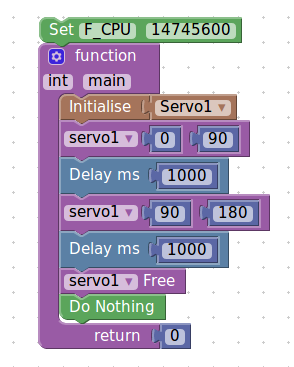
\includegraphics[scale =0.6]{servosam}\\[.3in]
    \textbf{Servo Motor}\\[1.3in]
    \end{center}
    
    
\newpage\section{Assembly of Hardware and Software}
%Circuit diagram and Steps of assembly of hardware with pictures for each step
\subsection*{Main Board Layout}
%Circuit schematic, simplified circuit diagram , block diagram of system
 \\\hfill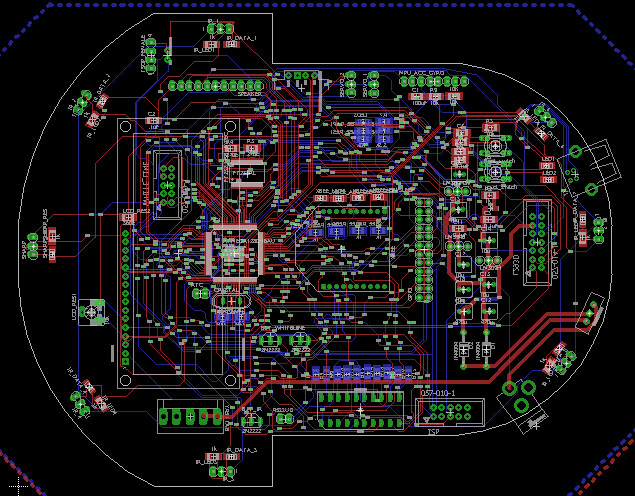
\includegraphics[width=14cm, height=11cm]{mainbrd}
 \caption{Fig 1.4A}
\subsection*{Step 1}
Collecting and purchasing all the components as specified in the List of Hardware table. Preparing the Schematic and Board Layout.
\subsection*{Step 2}
Solder the main PCB. Fig 1.4A shows the Main Board Layout.
\subsection*{Step 3}
Solder the modular PCB's. For instance Speaker. Fig 1.4B shows the board layout of Speaker, which needs to be soldered.
\\\hfill\includegraphics[width=14cm, height=11cm]{spkbrd}
 \caption{Fig 1.4B}
\subsection*{Step 4}
Attach the modular PCB's on to the main PCB, according to the functionality required.
\subsection*{Step 5}
Design the Algorithm of the code the user wishes to execute and place blocks accordingly on the localhost website. 
\subsection*{Step 6}
The user can see the Embedded C code of the algorithm created through blocks, on clicking FirebirdV button.
\subsection*{Step 7}
Generate the Hex File by clicking the Execute button.
\subsection*{Step 8}
Burn this Hex File on the Main Bot and run the code.


\section{Software and Code}

\href{http://www.github.com}{Github link} for the repository of code\\
Brief explanation of various parts of code 
\begin{enumerate}
    \item blocks.js\\
    This code comprises of the language code generated from Google Block Factory(Javascipt/JSON).
    \item blocks.blade.php\\
    This code comprises of the "Category ID" and the "Block type" which has to be defined by the user. The number of Block types would decide the number of sub-blocks in a main Block. The Block type corresponds to the name of the function generated in the Generator Stub of the Google Block Factory.
    \item fireblock.blade.php\\
    This file is used to specify the path of the blocks.js file.
    \item code.js
    The Category ID's defined in blocks.blade.php has to be inserted in the var categories[] list.\\
    eg var categories = ['catSensor']
    \item en.js
    The newly defined Category ID's have to be inserted here along with the name of the block, which would be displayed.\\
    eg. catSensor: "Sensor",
    \item generator.js
    This file corresponds to the Generator Stub of the google blockly code along with the embedded C coding generated at the backend.
    \item firebird.h
    This again consists of the embedded C code, this time along with the header files and the globally defined variables.
    \item ParseController.php
    This file is used for parsing where the PHP parsing code for XML is written.
\end{enumerate}

\textbf{User Instructions for demonstration}
\begin{enumerate}
    \item Create the blocks according to the algorithm of the code. This is done by "Drag and Drop" method. The "Thrash Button" has been created to remove unwanted blocks.
    \item The FirebirdV code(embedded C code) can be seen on clicking the FirebirdV button.
    \item The hex file of the code is generated by clicking the Execute button, which can be downloaded.
    \item Attach the modular bots needed to run this algorithm
    \item Burn this code on the miniBot and restart. The Bot would perform the required function.
\end{enumerate}

\href{http://www.youtube.com}{Youtube Link} of demonstration video 

\section{Future Work}
%What can be done to take this work ahead in future as projects.
 This application has a very wide scope.
  \begin{itemize}
   \item Automatic Hex Loading on the Robot from the Server.
   \item Addition of more abstraction for easier understanding.
   \item More useful blocks and functionality.
  \end{itemize}
\begin{thebibliography}{li}
%\bibitem{wavelan97}
%Ad Kamerman and Leo Monteban,
%{\em WaveLAN-II: A High-Performance Wireless LAN for the Unlicensed band},
%1997.
\bibitem{wavelan97}
Laravel Documentation:\href{http://laravel.com/docs/5.0}{http://laravel.com/docs/5.0} 
\bibitem{wavelan97}
Hex File Generation:\href{http://www.engineersgarage.com/forums/avr/how-generate-hex-file-using-avr-gcc-commands}{http://www.engineersgarage.com/forums/avr/how-generate-hex-file-using-avr-gcc-commands} 
\bibitem{wavelan97}
For PHP parsing refer:\href{http://php.net/manual/en/class.domdocument.php}{http://php.net/manual/en/class.domdocument.php} 
\bibitem{wavelan97}
To understand tree structure of xml:\href{http://www.w3schools.com/xml/xml\_tree.asp}{http://www.w3schools.com/xml/xml\_tree.asp} 
\bibitem{wavelan97}
 To understand javascript parsing:\href{http://www.w3schools.com/xml/xml\_parser.asp}{http://www.w3schools.com/xml/xml\_parser.asp} 
\bibitem{wavelan97}
To make blocks:\href{https://blockly-demo.appspot.com/static/demos/blockfactory/index.html}{https://blockly-demo.appspot.com/static/demos/blockfactory/index.html} 
\bibitem{wavelan97}
Blockly:\href{https://developers.google.com/blockly/custom-blocks/block-factory}{https://developers.google.com/blockly/custom-blocks/block-factory} 
\bibitem{wavelan97}
Save and upload file:\href{https://developer.mozilla.org/en/docs/Web/API/FileReader}{https://developer.mozilla.org/en/docs/Web/API/FileReader} 

\end{thebibliography}


\end{document}